\documentclass[tikz,border=3pt]{standalone}
\usepackage{amsmath}
\usepackage{tikz}
\usetikzlibrary{shapes.geometric,arrows.meta,patterns,calc}

\begin{document}
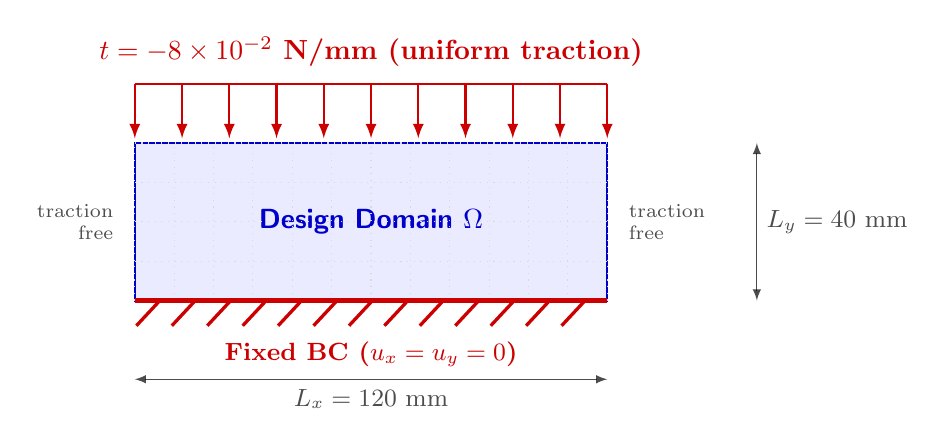
\begin{tikzpicture}[scale=1.0, >=latex]
  % BearingDevice2d: 120 x 40 mm, 绘图比例 0.05 -> 6.0 x 2.0
  % Design Domain
  \draw[thick, fill=blue!8, draw=blue!80!black] (0,0) rectangle (6,2);
  \node[font=\bfseries\sffamily, color=blue!80!black] at (3,1) {Design Domain $\Omega$};

  % Grid overlay
  \draw[step=0.5, gray!30, dotted] (0,0) grid (6,2);

  % Uniform distributed traction on the whole Top Edge (y = 40)
  \draw[thick, red!80!black] (0, 2.75) -- (6, 2.75);
  \foreach \x in {0.0, 0.6, 1.2, 1.8, 2.4, 3.0, 3.6, 4.2, 4.8, 5.4, 6.0} {
    \draw[->, thick, red!80!black] (\x, 2.75) -- (\x, 2.06);
  }
  \node[above, red!80!black, font=\bfseries] at (3, 2.85) {$t = -8\times 10^{-2}\text{ N/mm}$ (uniform traction)};

  % Fully clamped Bottom Edge (y = 0): u_x = u_y = 0
  \draw[ultra thick, red!80!black] (0,0) -- (6,0);
  \foreach \x in {0.3, 0.75, 1.2, 1.65, 2.1, 2.55, 3.0, 3.45, 3.9, 4.35, 4.8, 5.25, 5.7} {
    \draw[line width=1.2pt, red!80!black] (\x, -0.02) -- (\x-0.28, -0.32);
  }
  \node[below, red!80!black, font=\small\bfseries] at (3, -0.4) {Fixed BC ($u_x = u_y = 0$)};

  % Traction-free sides
  \node[left, gray!60!black, font=\scriptsize, align=right] at (-0.15, 1) {traction\\free};
  \node[right, gray!60!black, font=\scriptsize, align=left] at (6.15, 1) {traction\\free};

  % Dimensions
  \draw[<->, opacity=0.7] (0,-1.0) -- (6,-1.0) node[midway, below, font=\small] {$L_x = 120\text{ mm}$};
  \draw[<->, opacity=0.7] (7.9,0) -- (7.9,2) node[midway, right, font=\small] {$L_y = 40\text{ mm}$};
\end{tikzpicture}
\end{document}
